\documentclass{article}
\usepackage{tikz}
\usepackage{pgfplots}
\usepackage{textcomp}
\usepackage{array}
\usepackage{tabu}
\usepackage{numprint}
\usepackage{amsmath}
\usepackage{amssymb}
\usepackage{mathtools}
\usepackage{graphicx}
\graphicspath{{./}}
\DeclarePairedDelimiterX{\infdivx}[2]{(}{)}{%
  #1\;\delimsize\|\;#2%
}
\newcommand{\infdiv}{D\infdivx}
\DeclarePairedDelimiter{\norm}{\lVert}{\rVert}

\begin{document}


\title{Loss Analysis of Denoising Autoencoders on Gene Expression Data}
\section{Introduction}

\section{Gene Expression}
The abundance of spliced mRNA that is produced in a cell is referred to as the level of gene expression, which is a function of the rate of synthhesis of new mRNA and of its degradation.  \\
Because RNA levels are tightly controlled, measuring the concentrations of RNA found at a particular time and in a specific cell or organ can provide important information as to the function of the genes that encode them. In addition, the profile of RNAs found in a particular cell can be used as a means of disease diagnosis. For example, different types of cancer have been shown to have different RNA profiles. \\
Several different ways have been developed to deterine the RNA expression levels of all genes in the genome, called genome-wide expression analysis. \\
The data used for this study was collected using RNA-Seq. \\
The process o generating genome-wide information on RNA levels using sequencing is known as RNA-Seq. \\
\section{RNA-Seq}

\section{The Data}
The data was taken from the Genotype-Tissue Expression (GTEx) database. The data consits of genome-wide profiles of 2921 cells and perturbations.\\

\section{Autoencoders}
An autoencoder neural network is an unsupervised learning algorithm that applies backpropagation, setting the target values to be equal to the inputs. In other words, it tries to learn an approximation to the identity function. The identity function seems a particularly trivial function to be trying to learn; but by placing constraints on the network, such as by limiting the number of hidden units, we can discover interesting structure about the data. If we impose a "sparsity" constraint on the hidden units, then the autoencoder will still discover interesting strucutre in the data, even if the number of hidden units is large.\\

Let,
\begin{equation}
\hat{\rho}_j = \frac{1}{m} \sum_{i=1}^m [a^{(2)}_j(x^{(i)}) ]\\
\end{equation}
be the average activation of hidden unit $j$ (averaged over the training set). We would like to (approximately) enforce the constraint
\begin{equation}
\hat{\rho} = \rho,
\end{equation}
where $\rho$ is a "sparsity parameter", typically a small value close to zero (say $\rho = 0.05$). In other words, we would like the average activation of each hidden neuron $j$ to be close to 0.05 (say). To satisfy this constraint, the hidden unit's activations must mostly be near 0.\\
To achieve this, we will add an extra penalty term to our optimization objective that penalizes $\hat{\rho}_j$ deviating significantly from $\rho$. Many choices of the penalty term will give reasonable results. We will choose the following:\\

\begin{equation}
\sum_{j=1}^{s_2} \rho \log \frac{\rho}{\hat{\rho}_j} + (1 - \rho) \log \frac{1 - \rho}{1 - \hat{\rho}_j}
\end{equation}
Here, $s_2$ is the number of neurons in the hidden layer, and the index j is summing over the hidden units in our network.\\
This penalty term is based on KL divergence, and can be written 
\begin{equation}
\sum_{j=1}^{s_2}KL(\infdiv{\rho}{\hat{\rho}_j}),
\end{equation}
where
\begin{equation}
KL(\infdiv{\rho}{\hat{\rho}_j}) = \rho \log \frac{\rho}{\hat{\rho}_j} + (2 - \rho) \log \frac{1-\rho}{1-\hat{\rho}_j}
\end{equation}
is the Kullback-Leibler (KL) divergence between a Bernoulli random variable with mean $\rho$ and a Bernoulli random variable with mean $\rho_j$. KL-divergence is a standard function for measuring how different two different distributions are. This penalty function has the property that $KL(\infdiv{\rho}{\hat{\rho}_j}) = 0$ if $\hat{\rho}_j = \rho$, and otherwise it increases monotonically as $\hat{\rho}_j$ diverges from $\rho$.\\

For example, in the figure below, we have set $\rho = 0.2$,  and plotted $KL(\infdiv{\rho}{\hat{\rho}_j})$ for a range of values of $\hat{\rho}_j$.

\includegraphics[scale=0.5]{KLPenaltyExample}

We see that the KL-divergence reaches its minimum of 0 at\\
\begin{equation}
\hat{\rho}_j = \rho,
\end{equation}
and approaches $\inf$ as $\hat{\rho}_j$ approaches 0 or 1.

 


Our overall cost function is now,
\begin{equation}
J_{sparse}(W,b) = J(W,b)+ \beta \sum_{j=1}^{s_2}KL(\infdiv{\rho}{\hat{\rho}_j})
\end{equation}
where $J(W,b)$ is the loss function, and $\beta$ controls the weight of the sparsity penalty term.\\

\section{Denoising Autoencoder}
We test the performace of autoencoders in denoising gene expression data. Loss data from autoencoders of various depths was collected. Furthermore, loss was also measured as a function of the number of samples fed into the Autoencoder.\\
Loss was also calculated as a function of the amount of noise in the data.\\


\section{Deep Convolutional Autoencoder}
A deep convolutional autoencoder is an autoencoder that has convolutional layers. Convolutional autoencoders are popular and perform well in computer vision tasks. This is because images have the property that similar data is spatially nearby. Convolutional neural networks exploit this property and each convolutional filter learns a feature of the image, such as edges or eyes.\\
To test whether there is a correlation between spatial distance of the data and gene expression value, the deep convolutional data was collected and compared with a regular deep autoencoder of the same depth.  


\section{Calculation of Loss}
Let the number of samples be $N$, and let the number of genes (or the size of the sample) profiled in each sample be $M$. There are $N = 2921$ samples in the dataset, each sample profiled $M = 943$ genes, known as the L1000 genes, on a given cell and perturbation. Let the set of all samples be $S$, where 

\begin{equation}
  S = \{s_i \mid i \in [0, N), s_i \in \mathbb{R}^M\}
\end{equation}

We use additive Gaussian white noise to add noise into our dataset using the following equation:\\

\begin{equation}
s^\prime_{ij} = s_{ij} + \alpha \mathcal{N}(0,1)
\end{equation}

$s^\prime_{ij}$ is the profile for the i'th sample and the j'th gene, $\mathcal{N}(0,1)$ is the normal gaussian random variable, and $\alpha$ is the noise factor.\\
Therefore, the noisy set is defined as:\\

\begin{equation}
S^\prime = \{s^\prime_i \mid i \in [0,N)\}
\end{equation} 

And we define the Mean Square Error or MSE between the set $S$ and $S^\prime$ as follows: 
\begin{equation}
MSE(S,S^\prime) = \frac{1}{MN} \sum_{i=0, j=0}^{M, N}(s_{ij}-s^\prime_{ij})^{2}
\end{equation}

\section{Results}


\section{Discussion}
As the number of samples increases, the average mean square error goes down. 


\newpage

\bibliography{writeup}
\bibliographystyle{ieeetr}

\section{Appendix}

\subsection{1 layer Autoencoder}
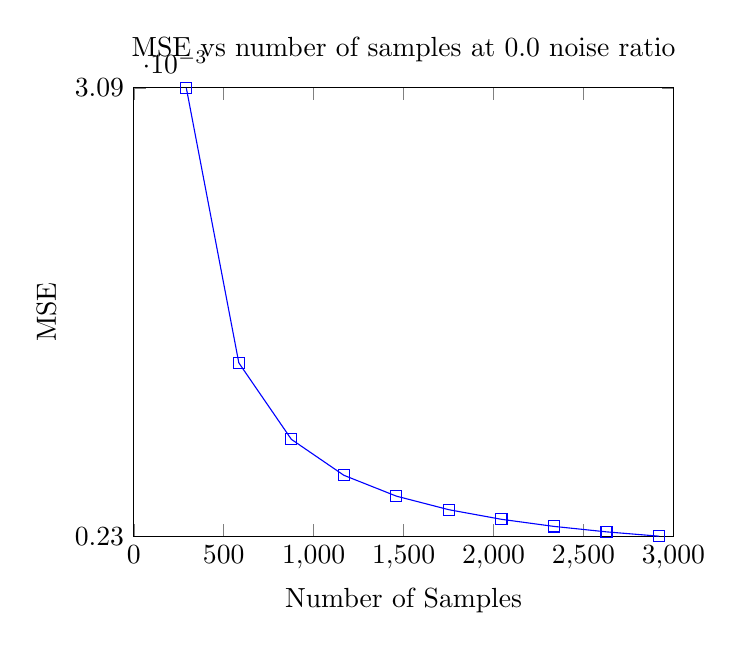
\begin{tikzpicture}
\begin{axis}[
title={MSE vs number of samples at  0.0 noise ratio},
xlabel={Number of Samples},
ylabel={MSE},
xmin=0, xmax=3000,
ymin=0.0002328581144910319, ymax=0.003086614669553874,
xtick={0,500,1000,1500,2000,2500,3000},
ytick={0.0002328581144910319,0.003086614669553874,0.005940371224616716,0.008794127779679558,0.0116478843347424,0.014501640889805241,0.01735539744486808,0.020209153999930923,0.023062910554993765,0.025916667110056607,0.02877042366511945},
legend pos=north west,
ymajorgrids=true,
grid style=dashed,
]

\addplot[
color=blue,
mark=square,
]
coordinates {

(292, 0.003086614669553874)
(584, 0.0013360799560614399)
(876, 0.0008494330624182567)
(1168, 0.0006204904244081578)
(1460, 0.00048774486070666195)
(1752, 0.0004013650028009695)
(2044, 0.00034033002267095205)
(2336, 0.00029513799870315994)
(2628, 0.0002604240402502465)
(2921, 0.0002328581144910319)
    };
\end{axis}
\end{tikzpicture}

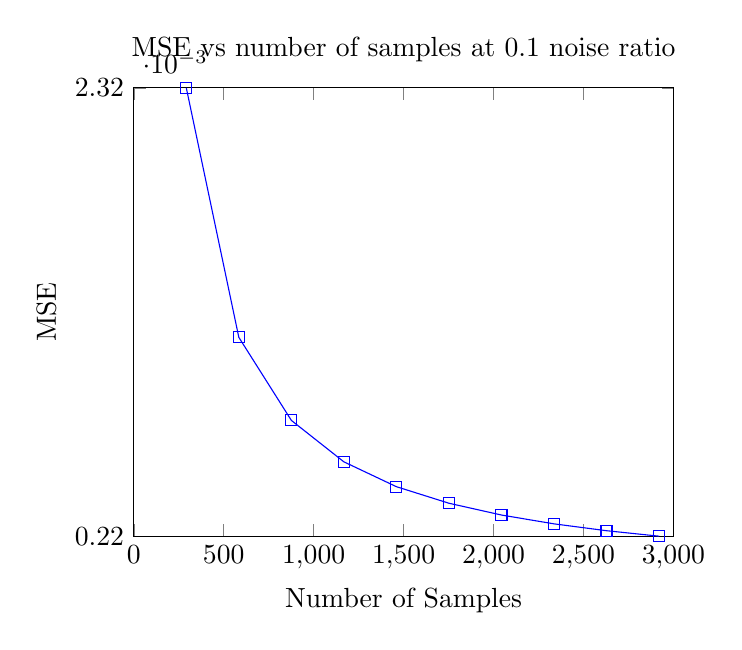
\begin{tikzpicture}
\begin{axis}[
title={MSE vs number of samples at  0.1 noise ratio},
xlabel={Number of Samples},
ylabel={MSE},
xmin=0, xmax=3000,
ymin=0.00022465084378037916, ymax=0.0023160638251677928,
xtick={0,500,1000,1500,2000,2500,3000},
ytick={0.00022465084378037916,0.0023160638251677928,0.004407476806555206,0.00649888978794262,0.008590302769330033,0.010681715750717446,0.012773128732104861,0.014864541713492274,0.016955954694879687,0.0190473676762671,0.021138780657654514},
legend pos=north west,
ymajorgrids=true,
grid style=dashed,
]

\addplot[
color=blue,
mark=square,
]
coordinates {

(292, 0.0023160638251677928)
(584, 0.0011523259998881604)
(876, 0.000764891884999634)
(1168, 0.0005715108915312078)
(1460, 0.0004556279897676719)
(1752, 0.00037842101031631)
(2044, 0.000323432708143004)
(2336, 0.0002822557279356208)
(2628, 0.00025026188006283646)
(2921, 0.00022465084378037916)
    };
\end{axis}
\end{tikzpicture}

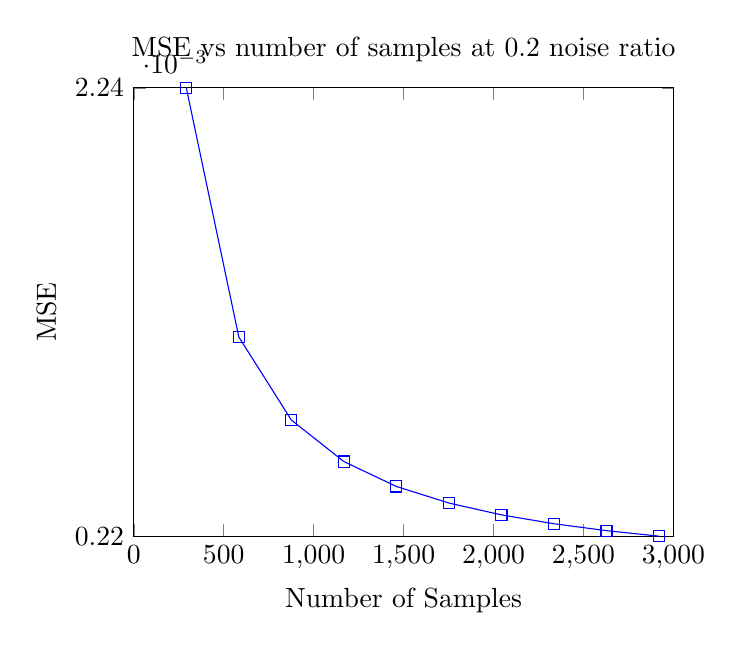
\begin{tikzpicture}
\begin{axis}[
title={MSE vs number of samples at 0.2 noise ratio},
xlabel={Number of Samples},
ylabel={MSE},
xmin=0, xmax=3000,
ymin=0.0002209009748328152, ymax=0.0022425452475827957,
xtick={0,500,1000,1500,2000,2500,3000},
ytick={0.0002209009748328152,0.0022425452475827957,0.004264189520332777,0.006285833793082758,0.008307478065832737,0.010329122338582717,0.012350766611332699,0.014372410884082679,0.01639405515683266,0.01841569942958264,0.02043734370233262},
legend pos=north west,
ymajorgrids=true,
grid style=dashed,
]

\addplot[
color=blue,
mark=square,
]
coordinates {

(292, 0.0022425452475827957)
(584, 0.0011190090358605491)
(876, 0.0007446046341546937)
(1168, 0.0005573554281322452)
(1460, 0.00044512918843772376)
(1752, 0.0003703706431465638)
(2044, 0.00031698772717414416)
(2336, 0.00027697729949968203)
(2628, 0.0002458468506690461)
(2921, 0.0002209009748328152)
    };
\end{axis}
\end{tikzpicture}

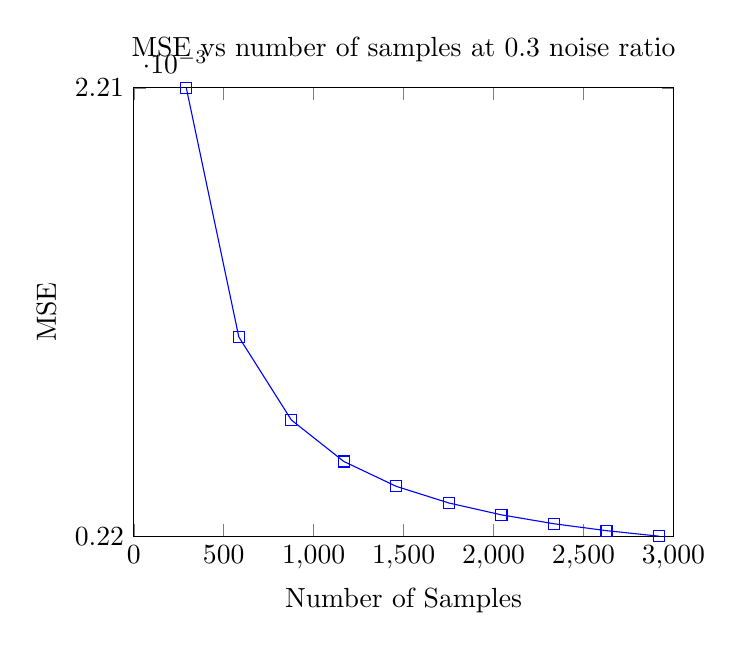
\begin{tikzpicture}
\begin{axis}[
title={MSE vs number of samples at 0.3 noise ratio},
xlabel={Number of Samples},
ylabel={MSE},
xmin=0, xmax=3000,
ymin=0.0002186491313732399, ymax=0.002206864060481076,
xtick={0,500,1000,1500,2000,2500,3000},
ytick={0.0002186491313732399,0.002206864060481076,0.004195078989588912,0.006183293918696748,0.008171508847804584,0.01015972377691242,0.012147938706020257,0.014136153635128093,0.01612436856423593,0.018112583493343763,0.0201007984224516},
legend pos=north west,
ymajorgrids=true,
grid style=dashed,
]

\addplot[
color=blue,
mark=square,
]
coordinates {

(292, 0.002206864060481076)
(584, 0.001102091101842601)
(876, 0.0007339627647133898)
(1168, 0.0005499236199411678)
(1460, 0.00043948317300785745)
(1752, 0.0003658850356728808)
(2044, 0.00031329472053076026)
(2336, 0.0002738564656156271)
(2628, 0.00024322542142790152)
(2921, 0.0002186491313732399)
    };
\end{axis}
\end{tikzpicture}

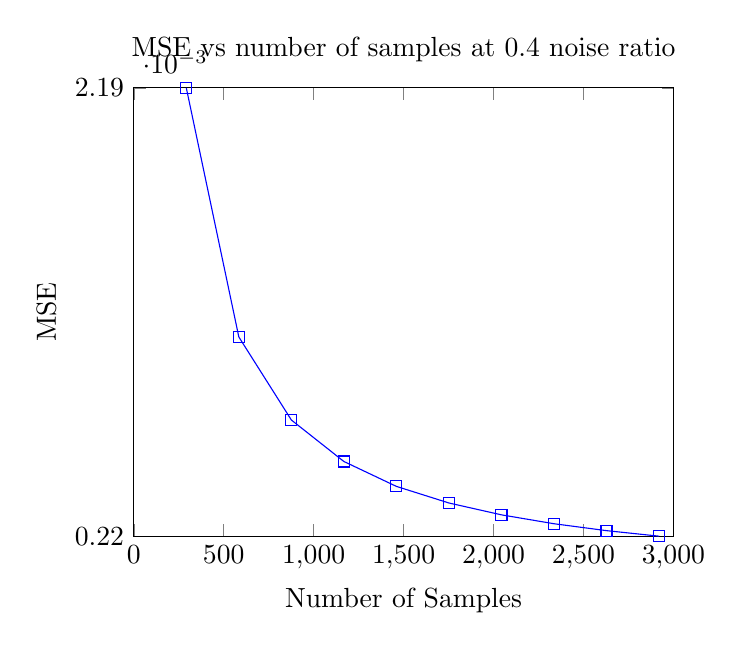
\begin{tikzpicture}
\begin{axis}[
title={MSE vs number of samples at 0.4 noise ratio},
xlabel={Number of Samples},
ylabel={MSE},
xmin=0, xmax=3000,
ymin=0.00021715967007732436, ymax=0.0021854388898646018,
xtick={0,500,1000,1500,2000,2500,3000},
ytick={0.00021715967007732436,0.0021854388898646018,0.0041537181096518785,0.006121997329439156,0.008090276549226434,0.01005855576901371,0.01202683498880099,0.013995114208588266,0.015963393428375543,0.01793167264816282,0.019899951867950096},
legend pos=north west,
ymajorgrids=true,
grid style=dashed,
]

\addplot[
color=blue,
mark=square,
]
coordinates {

(292, 0.0021854388898646018)
(584, 0.001091781887639273)
(876, 0.000727338326736149)
(1168, 0.0005451333720982601)
(1460, 0.00043578787350424445)
(1752, 0.00036290888494552767)
(2044, 0.00031087150212453135)
(2336, 0.0002718448167248128)
(2628, 0.00024150095415572499)
(2921, 0.00021715967007732436)
    };
\end{axis}
\end{tikzpicture}

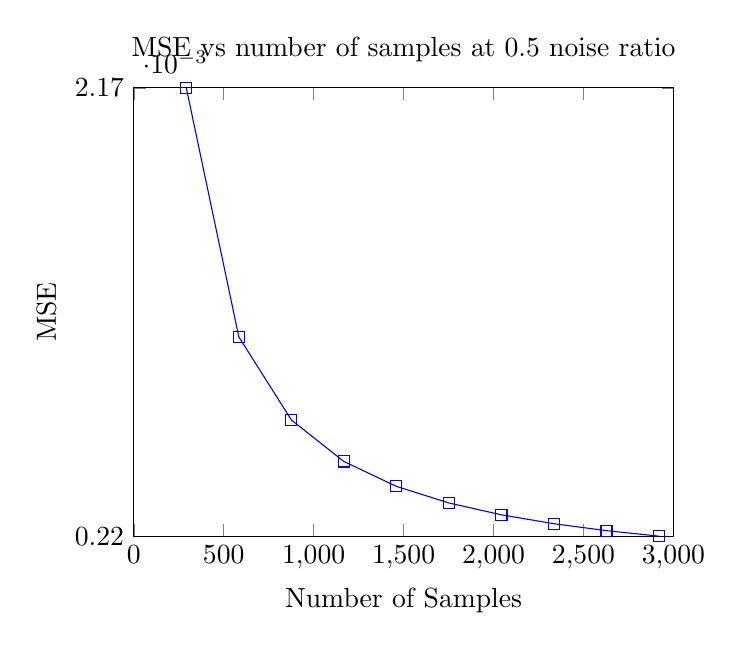
\begin{tikzpicture}
\begin{axis}[
title={MSE vs number of samples at 0.5 noise ratio},
xlabel={Number of Samples},
ylabel={MSE},
xmin=0, xmax=3000,
ymin=0.0002159982379709205, ymax=0.002170996633125675,
xtick={0,500,1000,1500,2000,2500,3000},
ytick={0.0002159982379709205,0.002170996633125675,0.004125995028280429,0.006080993423435183,0.008035991818589938,0.009990990213744692,0.011945988608899448,0.013900987004054201,0.015855985399208954,0.01781098379436371,0.01976598218951846},
legend pos=north west,
ymajorgrids=true,
grid style=dashed,
]

\addplot[
color=blue,
mark=square,
]
coordinates {

(292, 0.002170996633125675)
(584, 0.0010849836445733752)
(876, 0.0007229809024172386)
(1168, 0.0005418496509812905)
(1460, 0.00043327936234693133)
(1752, 0.0003608943044502226)
(2044, 0.0003091998683644169)
(2336, 0.00027033082249084344)
(2628, 0.00024018665583547337)
(2921, 0.0002159982379709205)
    };
\end{axis}
\end{tikzpicture}

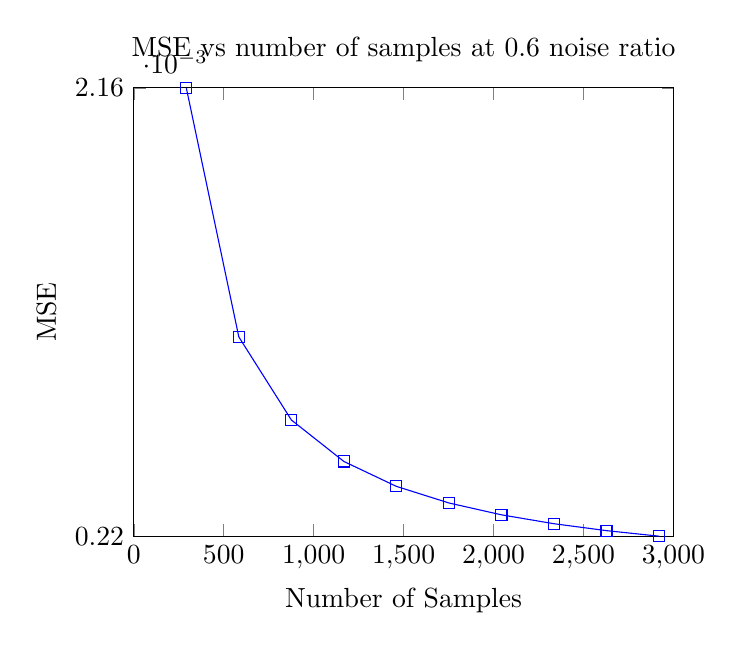
\begin{tikzpicture}
\begin{axis}[
title={MSE vs number of samples at 0.6 noise ratio},
xlabel={Number of Samples},
ylabel={MSE},
xmin=0, xmax=3000,
ymin=0.00021529969486119686, ymax=0.0021598107529969108,
xtick={0,500,1000,1500,2000,2500,3000},
ytick={0.00021529969486119686,0.0021598107529969108,0.004104321811132625,0.006048832869268338,0.007993343927404053,0.009937854985539767,0.01188236604367548,0.013826877101811194,0.01577138815994691,0.017715899218082625,0.01966041027621834},
legend pos=north west,
ymajorgrids=true,
grid style=dashed,
]

\addplot[
color=blue,
mark=square,
]
coordinates {

(292, 0.0021598107529969108)
(584, 0.0010795527510194362)
(876, 0.0007194600267083208)
(1168, 0.00053942483757223)
(1460, 0.0004313928480070553)
(1752, 0.0003593836164476067)
(2044, 0.0003079597281001374)
(2336, 0.00026938359259951464)
(2628, 0.00023938314403331283)
(2921, 0.00021529969486119686)
    };
\end{axis}
\end{tikzpicture}

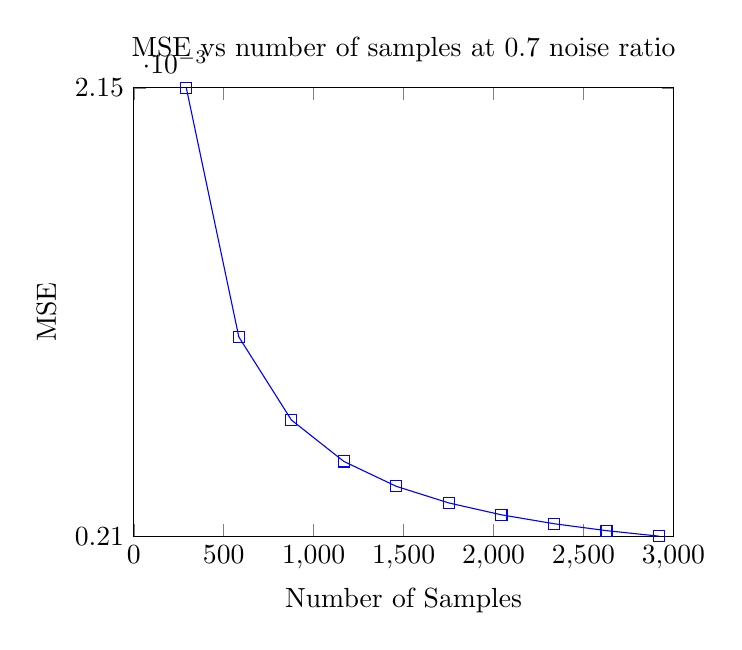
\begin{tikzpicture}
\begin{axis}[
title={MSE vs number of samples at 0.7 noise ratio},
xlabel={Number of Samples},
ylabel={MSE},
xmin=0, xmax=3000,
ymin=0.00021475981148318923, ymax=0.002152772841323252,
xtick={0,500,1000,1500,2000,2500,3000},
ytick={0.00021475981148318923,0.002152772841323252,0.004090785871163315,0.006028798901003377,0.00796681193084344,0.009904824960683503,0.011842837990523566,0.013780851020363628,0.01571886405020369,0.01765687708004375,0.019594890109883814},
legend pos=north west,
ymajorgrids=true,
grid style=dashed,
]

\addplot[
color=blue,
mark=square,
]
coordinates {

(292, 0.002152772841323252)
(584, 0.0010761141182642417)
(876, 0.0007172147254221748)
(1168, 0.0005378111133403794)
(1460, 0.00043012699295660043)
(1752, 0.0003583599054253409)
(2044, 0.00030709755960643437)
(2336, 0.00026866261170932753)
(2628, 0.00023875387962653973)
(2921, 0.00021475981148318923)
    };
\end{axis}
\end{tikzpicture}

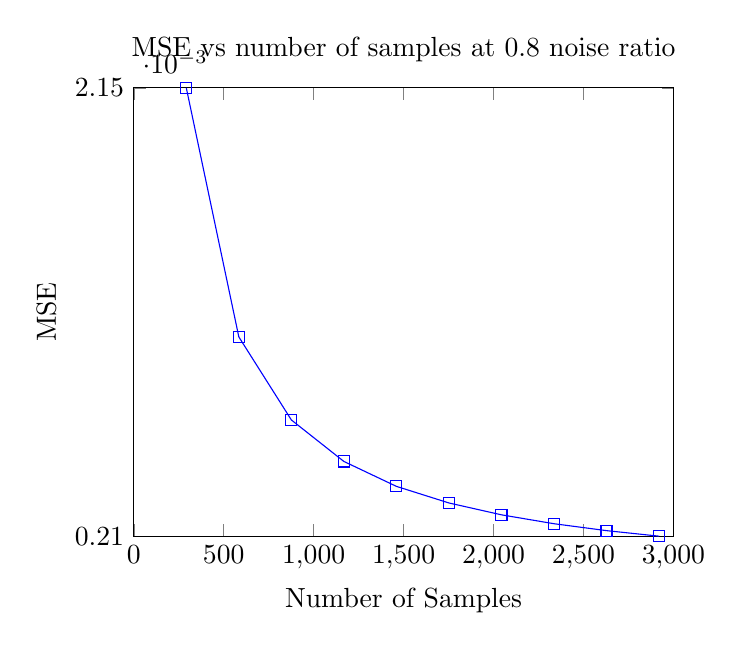
\begin{tikzpicture}
\begin{axis}[
title={MSE vs number of samples at 0.8 noise ratio},
xlabel={Number of Samples},
ylabel={MSE},
xmin=0, xmax=3000,
ymin=0.00021434921515361914, ymax=0.0021476378805090806,
xtick={0,500,1000,1500,2000,2500,3000},
ytick={0.00021434921515361914,0.0021476378805090806,0.004080926545864542,0.006014215211220003,0.007947503876575465,0.009880792541930927,0.011814081207286388,0.01374736987264185,0.01568065853799731,0.017613947203352773,0.019547235868708233},
legend pos=north west,
ymajorgrids=true,
grid style=dashed,
]

\addplot[
color=blue,
mark=square,
]
coordinates {

(292, 0.0021476378805090806)
(584, 0.0010736718065106473)
(876, 0.0007156397165912511)
(1168, 0.0005366461991449404)
(1460, 0.00042922981110524985)
(1752, 0.00035763682457621177)
(2044, 0.0003064848368146558)
(2336, 0.00026812432054125674)
(2628, 0.00023829416561066088)
(2921, 0.00021434921515361914)
    };
\end{axis}
\end{tikzpicture}

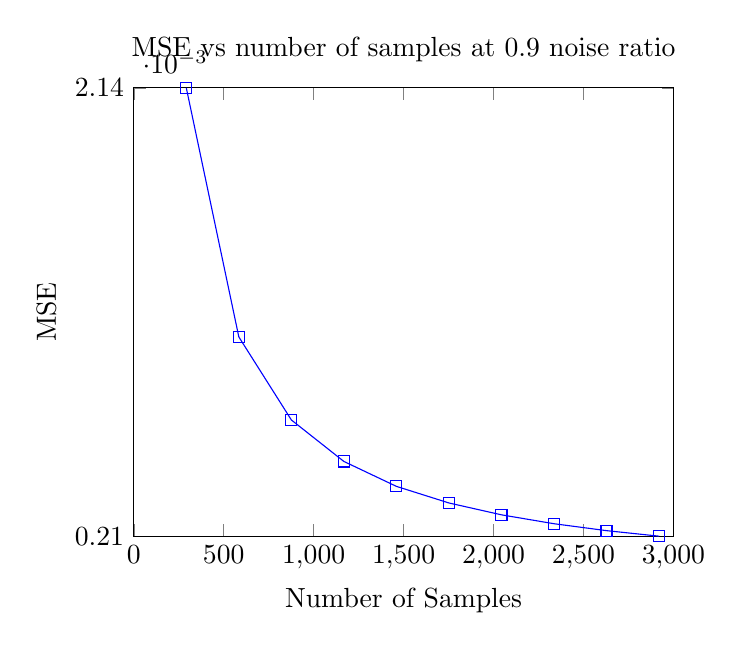
\begin{tikzpicture}
\begin{axis}[
title={MSE vs number of samples at 0.9 noise ratio},
xlabel={Number of Samples},
ylabel={MSE},
xmin=0, xmax=3000,
ymin=0.00021405789921874523, ymax=0.0021436493654317917,
xtick={0,500,1000,1500,2000,2500,3000},
ytick={0.00021405789921874523,0.0021436493654317917,0.004073240831644839,0.006002832297857885,0.00793242376407093,0.009862015230283978,0.011791606696497023,0.01372119816271007,0.015650789628923117,0.017580381095136162,0.01950997256134921},
legend pos=north west,
ymajorgrids=true,
grid style=dashed,
]

\addplot[
color=blue,
mark=square,
]
coordinates {

(292, 0.0021436493654317917)
(584, 0.0010716816046299911)
(876, 0.0007143846978303176)
(1168, 0.0005357529493844871)
(1460, 0.0004285467278133377)
(1752, 0.00035708138055920224)
(2044, 0.00030603608796304823)
(2336, 0.0002677401884786246)
(2628, 0.00023795709541679628)
(2921, 0.00021405789921874523)
    };
\end{axis}
\end{tikzpicture}

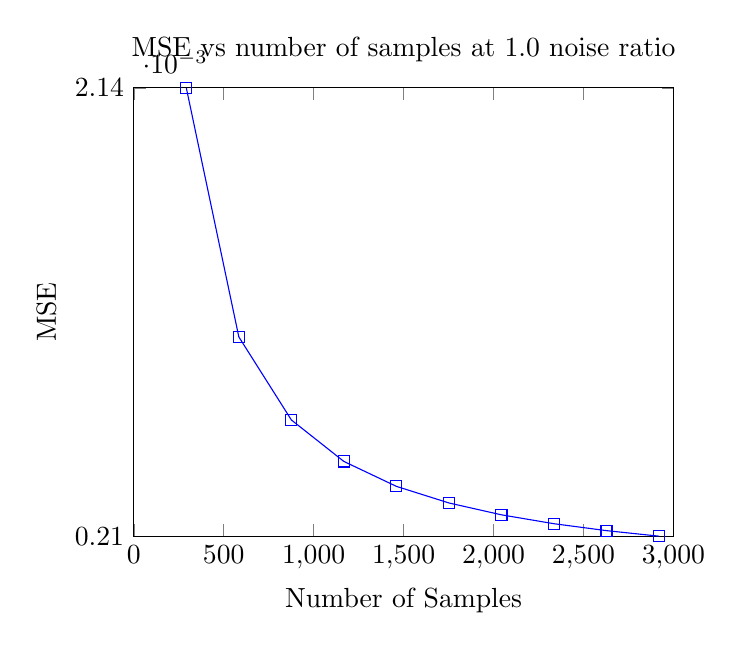
\begin{tikzpicture}
\begin{axis}[
title={MSE vs number of samples at 1.0 noise ratio},
xlabel={Number of Samples},
ylabel={MSE},
xmin=0, xmax=3000,
ymin=0.00021384841078681162, ymax=0.002140742636665644,
xtick={0,500,1000,1500,2000,2500,3000},
ytick={0.00021384841078681162,0.002140742636665644,0.004067636862544476,0.005994531088423309,0.007921425314302141,0.009848319540180972,0.011775213766059806,0.013702107991938639,0.01562900221781747,0.0175558964436963,0.01948279066957513},
legend pos=north west,
ymajorgrids=true,
grid style=dashed,
]

\addplot[
color=blue,
mark=square,
]
coordinates {

(292, 0.002140742636665644)
(584, 0.0010703501218532901)
(876, 0.0007135366658680865)
(1168, 0.0005351137998863384)
(1460, 0.0004280492255514533)
(1752, 0.00035668415170715087)
(2044, 0.00030569300621399167)
(2336, 0.0002674611527313564)
(2628, 0.0002377095549381096)
(2921, 0.00021384841078681162)
    };
\end{axis}
\end{tikzpicture}

\subsection{Two layer autoencoder}
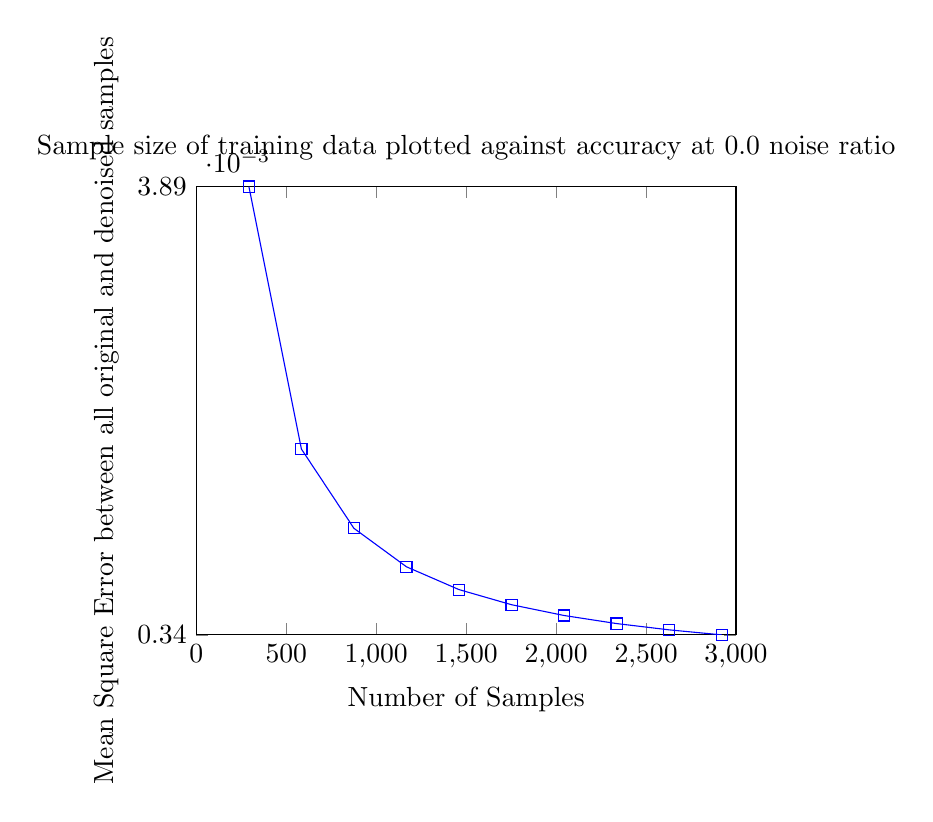
\begin{tikzpicture}
\begin{axis}[
title={Sample size of training data plotted against accuracy at 0.0 noise ratio},
xlabel={Number of Samples},
ylabel={Mean Square Error between all original and denoised samples},
xmin=0, xmax=3000,
ymin=0.00034263676416242225, ymax=0.003893047247220739,
xtick={0,500,1000,1500,2000,2500,3000},
ytick={0.00034263676416242225,0.003893047247220739,0.007443457730279056,0.010993868213337374,0.01454427869639569,0.018094689179454004,0.021645099662512324,0.02519551014557064,0.028745920628628956,0.032296331111687275,0.03584674159474559},
legend pos=north west,
ymajorgrids=true,
grid style=dashed,
]

\addplot[
color=blue,
mark=square,
]
coordinates {

(292, 0.003893047247220739)
(584, 0.0018143391836784833)
(876, 0.0011864803861535744)
(1168, 0.0008818756735305562)
(1460, 0.0007013013396741172)
(1752, 0.0005815588056184408)
(2044, 0.0004961894514461288)
(2336, 0.00043226203629193565)
(2628, 0.00038252136348554584)
(2921, 0.00034263676416242225)
    };
\end{axis}
\end{tikzpicture}

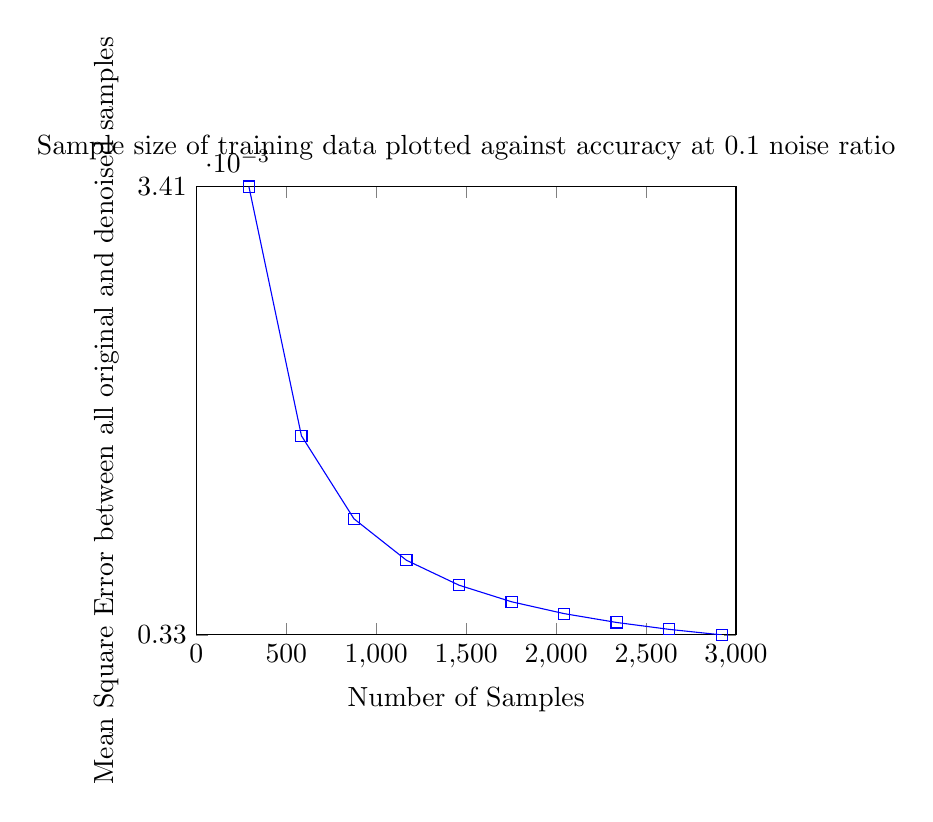
\begin{tikzpicture}
\begin{axis}[
title={Sample size of training data plotted against accuracy at 0.1 noise ratio},
xlabel={Number of Samples},
ylabel={Mean Square Error between all original and denoised samples},
xmin=0, xmax=3000,
ymin=0.0003290003792078779, ymax=0.0034125392408360486,
xtick={0,500,1000,1500,2000,2500,3000},
ytick={0.0003290003792078779,0.0034125392408360486,0.006496078102464219,0.00957961696409239,0.01266315582572056,0.01574669468734873,0.0188302335489769,0.02191377241060507,0.02499731127223324,0.028080850133861412,0.03116438899548958},
legend pos=north west,
ymajorgrids=true,
grid style=dashed,
]

\addplot[
color=blue,
mark=square,
]
coordinates {

(292, 0.0034125392408360486)
(584, 0.001698710423545089)
(876, 0.0011276105661451265)
(1168, 0.0008421620052160637)
(1460, 0.0006709262920575356)
(1752, 0.0005568437754745602)
(2044, 0.00047543099619836023)
(2336, 0.0004144384530961431)
(2628, 0.0003670187496604608)
(2921, 0.0003290003792078779)
    };
\end{axis}
\end{tikzpicture}

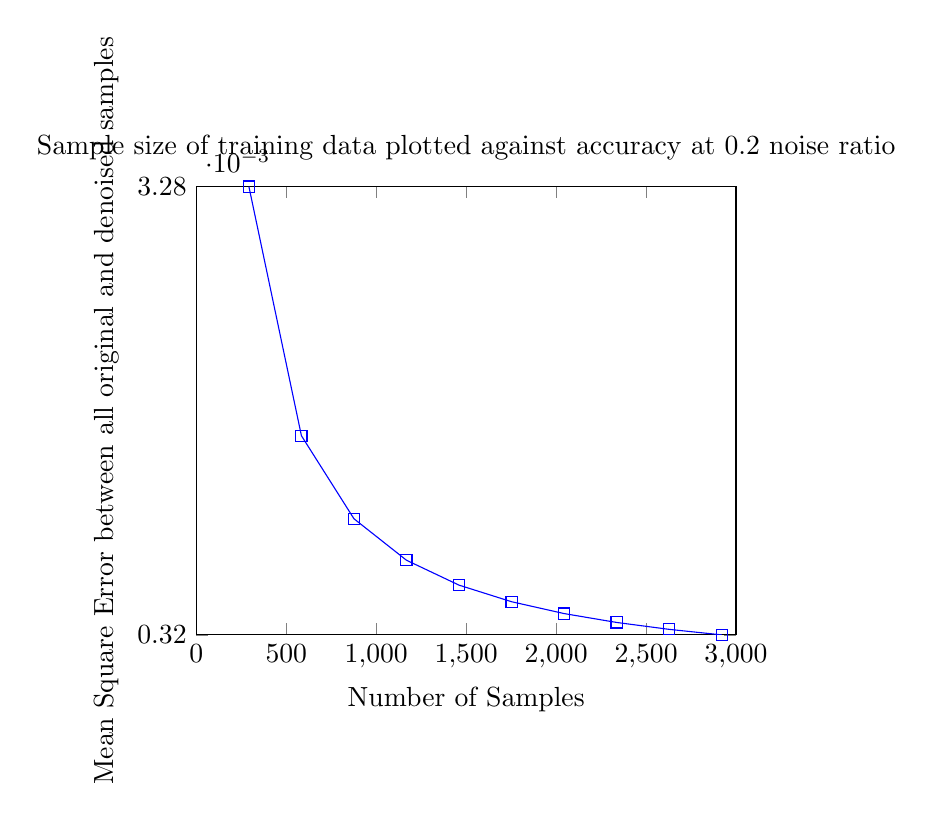
\begin{tikzpicture}
\begin{axis}[
title={Sample size of training data plotted against accuracy at 0.2 noise ratio},
xlabel={Number of Samples},
ylabel={Mean Square Error between all original and denoised samples},
xmin=0, xmax=3000,
ymin=0.0003179121409091245, ymax=0.003278955461346756,
xtick={0,500,1000,1500,2000,2500,3000},
ytick={0.0003179121409091245,0.003278955461346756,0.006239998781784387,0.009201042102222019,0.01216208542265965,0.015123128743097281,0.018084172063534912,0.021045215383972544,0.024006258704410175,0.026967302024847806,0.029928345345285438},
legend pos=north west,
ymajorgrids=true,
grid style=dashed,
]

\addplot[
color=blue,
mark=square,
]
coordinates {

(292, 0.003278955461346756)
(584, 0.0016333440079783028)
(876, 0.0010850142223081292)
(1168, 0.0008109602081382655)
(1460, 0.0006465648709210232)
(1752, 0.0005370156780768849)
(2044, 0.00045877337129718624)
(2336, 0.0004000497070222364)
(2628, 0.00035446392305861144)
(2921, 0.0003179121409091245)
    };
\end{axis}
\end{tikzpicture}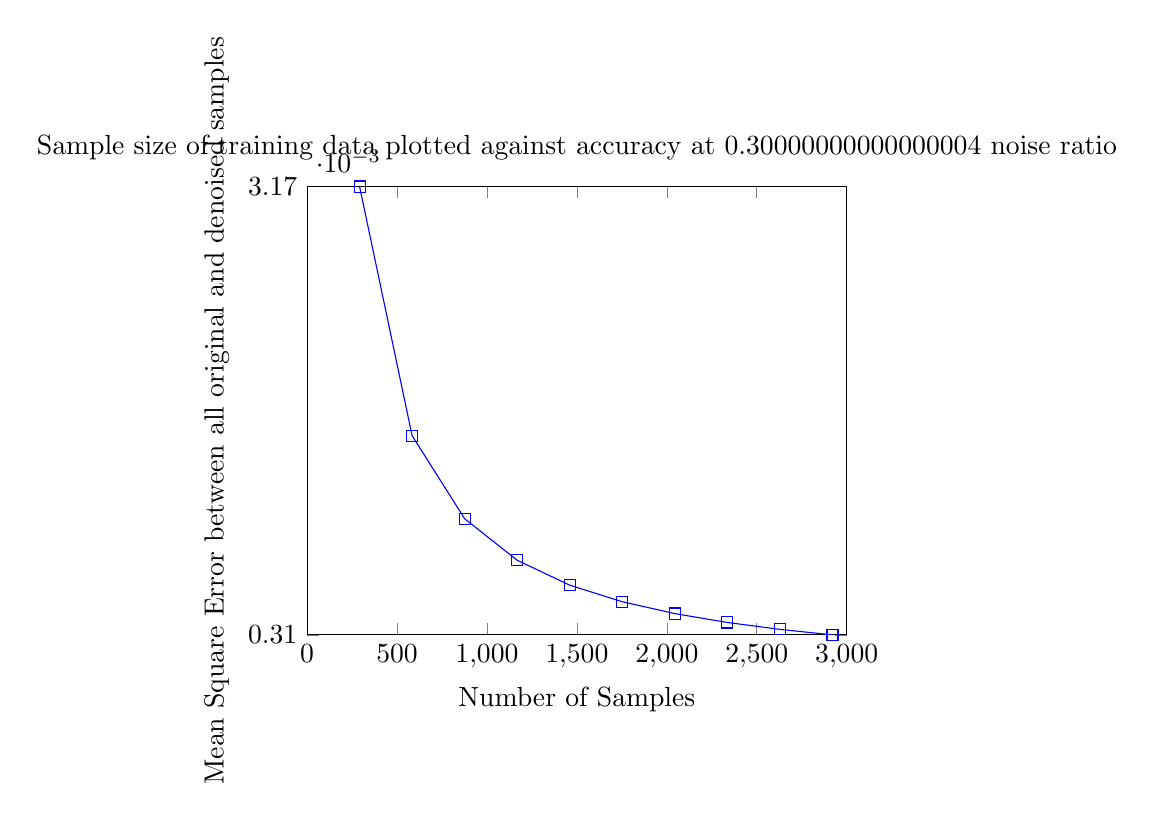
\begin{tikzpicture}
\begin{axis}[
title={Sample size of training data plotted against accuracy at 0.30000000000000004 noise ratio},
xlabel={Number of Samples},
ylabel={Mean Square Error between all original and denoised samples},
xmin=0, xmax=3000,
ymin=0.0003087277982890565, ymax=0.0031701273498587726,
xtick={0,500,1000,1500,2000,2500,3000},
ytick={0.0003087277982890565,0.0031701273498587726,0.006031526901428489,0.008892926452998206,0.011754326004567921,0.014615725556137637,0.017477125107707357,0.02033852465927707,0.023199924210846788,0.026061323762416506,0.02892272331398622},
legend pos=north west,
ymajorgrids=true,
grid style=dashed,
]

\addplot[
color=blue,
mark=square,
]
coordinates {

(292, 0.0031701273498587726)
(584, 0.0015800748662240102)
(876, 0.0010500288075128436)
(1168, 0.0007851058925674953)
(1460, 0.0006262207134368575)
(1752, 0.0005203444800839386)
(2044, 0.0004447511028264257)
(2336, 0.0003880948692040476)
(2628, 0.00034405555796425077)
(2921, 0.0003087277982890565)
    };
\end{axis}
\end{tikzpicture}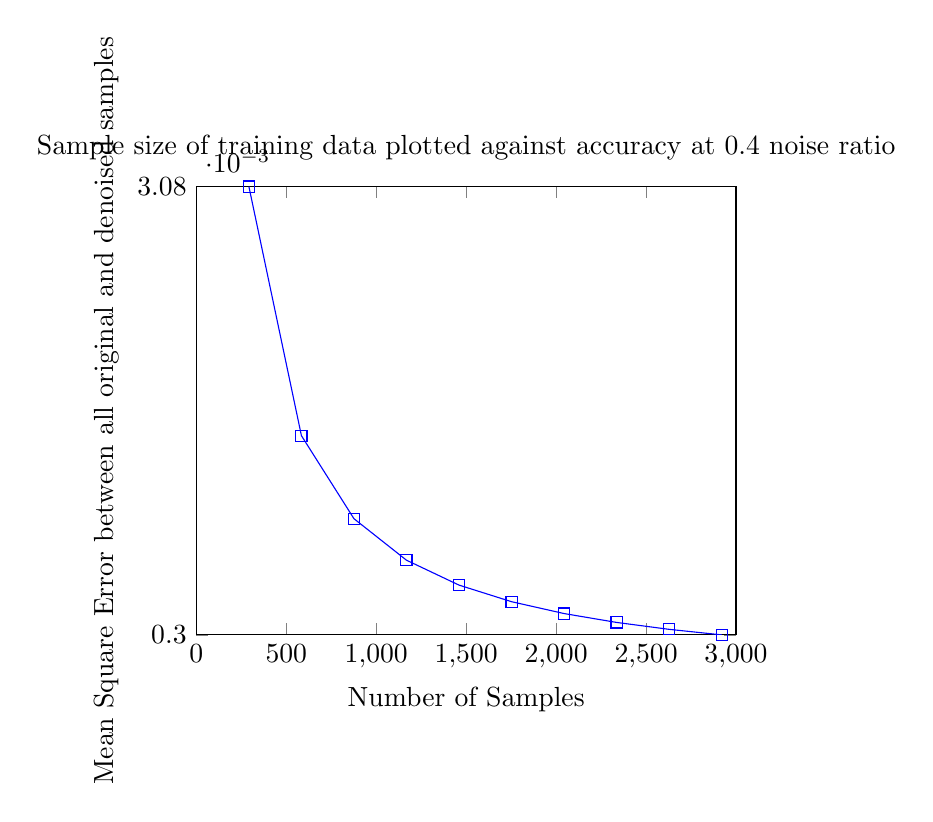
\begin{tikzpicture}
\begin{axis}[
title={Sample size of training data plotted against accuracy at 0.4 noise ratio},
xlabel={Number of Samples},
ylabel={Mean Square Error between all original and denoised samples},
xmin=0, xmax=3000,
ymin=0.00030146121510226515, ymax=0.0030803792528481116,
xtick={0,500,1000,1500,2000,2500,3000},
ytick={0.00030146121510226515,0.0030803792528481116,0.005859297290593958,0.008638215328339804,0.01141713336608565,0.014196051403831497,0.016974969441577344,0.01975388747932319,0.022532805517069036,0.025311723554814883,0.02809064159256073},
legend pos=north west,
ymajorgrids=true,
grid style=dashed,
]

\addplot[
color=blue,
mark=square,
]
coordinates {

(292, 0.0030803792528481116)
(584, 0.0015363670631329438)
(876, 0.001021713759896783)
(1168, 0.0007644402968804377)
(1460, 0.0006100843101925319)
(1752, 0.0005072031221733987)
(2044, 0.00043374137002942585)
(2336, 0.0003786697427381918)
(2628, 0.00033584611304254076)
(2921, 0.00030146121510226515)
    };
\end{axis}
\end{tikzpicture}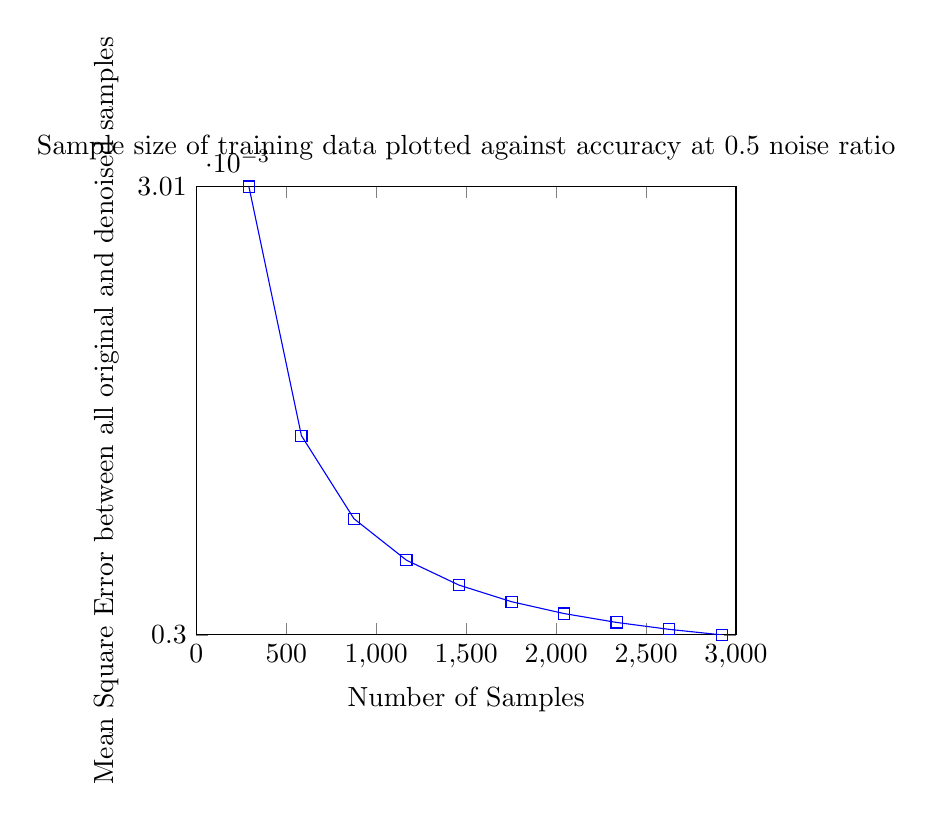
\begin{tikzpicture}
\begin{axis}[
title={Sample size of training data plotted against accuracy at 0.5 noise ratio},
xlabel={Number of Samples},
ylabel={Mean Square Error between all original and denoised samples},
xmin=0, xmax=3000,
ymin=0.00029523576996414466, ymax=0.003009049737509041,
xtick={0,500,1000,1500,2000,2500,3000},
ytick={0.00029523576996414466,0.003009049737509041,0.005722863705053938,0.008436677672598833,0.01115049164014373,0.013864305607688627,0.016578119575233523,0.01929193354277842,0.022005747510323317,0.024719561477868215,0.027433375445413112},
legend pos=north west,
ymajorgrids=true,
grid style=dashed,
]

\addplot[
color=blue,
mark=square,
]
coordinates {

(292, 0.003009049737509041)
(584, 0.0015011582659768458)
(876, 0.000998527414326503)
(1168, 0.0007472762388215044)
(1460, 0.0005965678610208354)
(1752, 0.0004961057257035968)
(2044, 0.0004243780929967037)
(2336, 0.0003705937963066777)
(2628, 0.0003287694927845347)
(2921, 0.00029523576996414466)
    };
\end{axis}
\end{tikzpicture}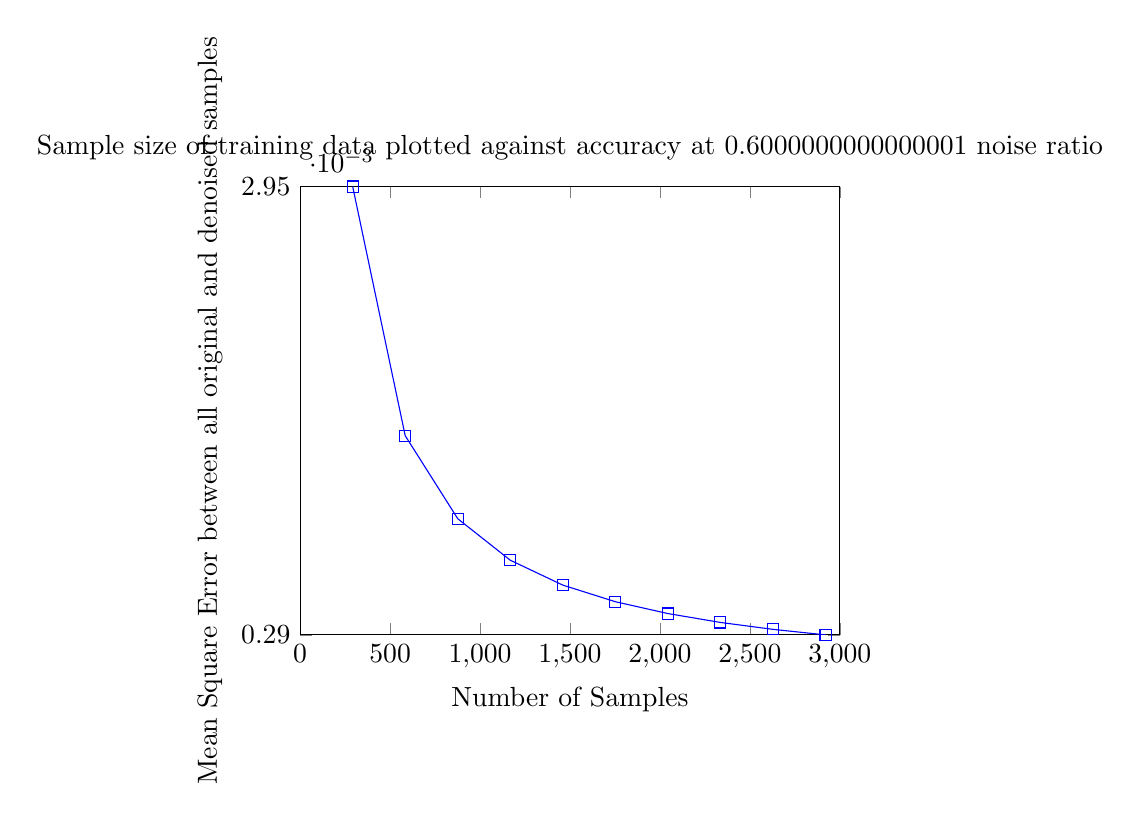
\begin{tikzpicture}
\begin{axis}[
title={Sample size of training data plotted against accuracy at 0.6000000000000001 noise ratio},
xlabel={Number of Samples},
ylabel={Mean Square Error between all original and denoised samples},
xmin=0, xmax=3000,
ymin=0.000289934068473812, ymax=0.002947796593034476,
xtick={0,500,1000,1500,2000,2500,3000},
ytick={0.000289934068473812,0.002947796593034476,0.00560565911759514,0.008263521642155804,0.010921384166716468,0.013579246691277132,0.016237109215837795,0.01889497174039846,0.021552834264959124,0.024210696789519787,0.026868559314080453},
legend pos=north west,
ymajorgrids=true,
grid style=dashed,
]

\addplot[
color=blue,
mark=square,
]
coordinates {

(292, 0.002947796593034476)
(584, 0.00147091923659838)
(876, 0.0009787701932290613)
(1168, 0.0007327538346160407)
(1460, 0.0005851367859140627)
(1752, 0.00048673417692110874)
(2044, 0.0004164763386878367)
(2336, 0.00036377907860995795)
(2628, 0.0003228042856227986)
(2921, 0.000289934068473812)
    };
\end{axis}
\end{tikzpicture}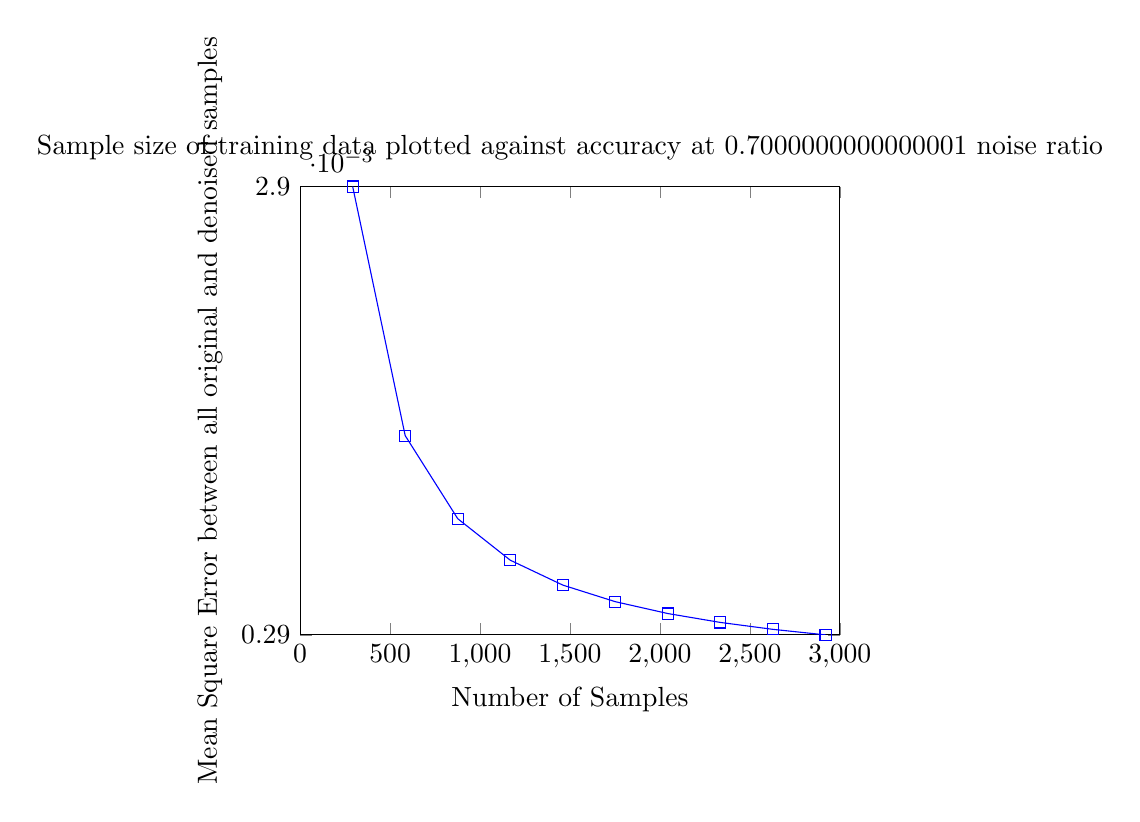
\begin{tikzpicture}
\begin{axis}[
title={Sample size of training data plotted against accuracy at 0.7000000000000001 noise ratio},
xlabel={Number of Samples},
ylabel={Mean Square Error between all original and denoised samples},
xmin=0, xmax=3000,
ymin=0.00028539912254076577, ymax=0.0028955197745405715,
xtick={0,500,1000,1500,2000,2500,3000},
ytick={0.00028539912254076577,0.0028955197745405715,0.005505640426540378,0.008115761078540184,0.01072588173053999,0.013336002382539795,0.0159461230345396,0.018556243686539405,0.02116636433853921,0.023776484990539016,0.02638660564253882},
legend pos=north west,
ymajorgrids=true,
grid style=dashed,
]

\addplot[
color=blue,
mark=square,
]
coordinates {

(292, 0.0028955197745405715)
(584, 0.0014453669031234985)
(876, 0.0009619898820102645)
(1168, 0.000720341226586597)
(1460, 0.0005753617281749155)
(1752, 0.00047872709928574263)
(2044, 0.00040970383128073937)
(2336, 0.00035794370940363886)
(2628, 0.00031769335197070017)
(2921, 0.00028539912254076577)
    };
\end{axis}
\end{tikzpicture}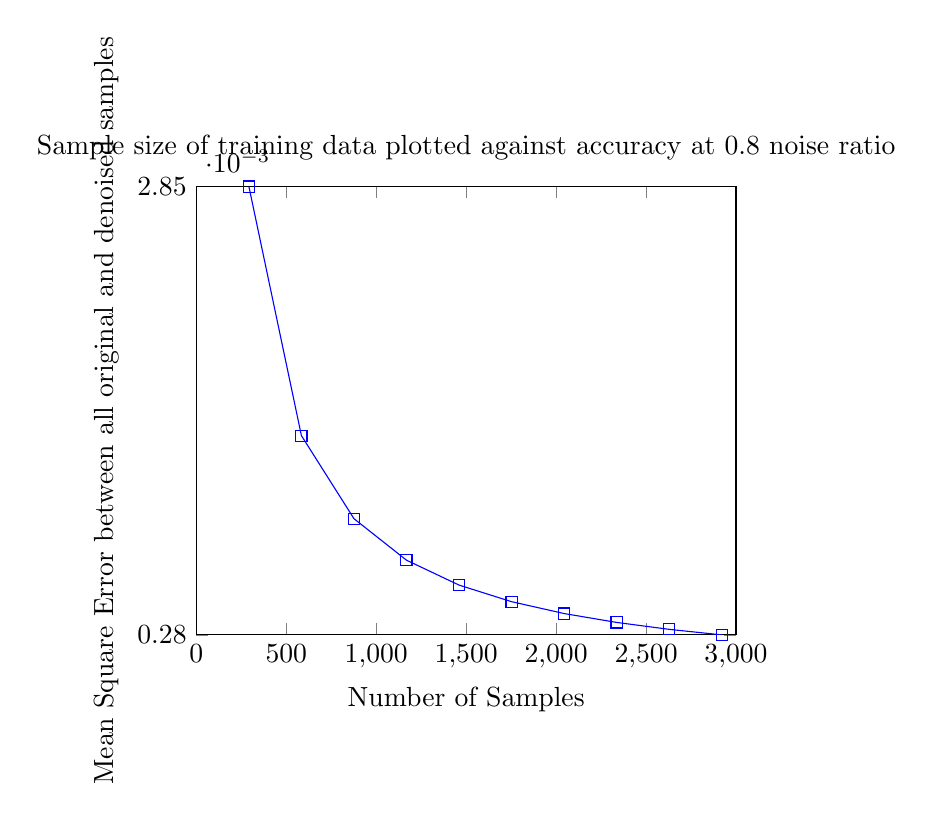
\begin{tikzpicture}
\begin{axis}[
title={Sample size of training data plotted against accuracy at 0.8 noise ratio},
xlabel={Number of Samples},
ylabel={Mean Square Error between all original and denoised samples},
xmin=0, xmax=3000,
ymin=0.0002813744141666843, ymax=0.0028507990231257207,
xtick={0,500,1000,1500,2000,2500,3000},
ytick={0.0002813744141666843,0.0028507990231257207,0.005420223632084757,0.007989648241043793,0.01055907285000283,0.013128497458961866,0.0156979220679209,0.018267346676879938,0.020836771285838974,0.02340619589479801,0.025975620503757048},
legend pos=north west,
ymajorgrids=true,
grid style=dashed,
]

\addplot[
color=blue,
mark=square,
]
coordinates {

(292, 0.0028507990231257207)
(584, 0.0014233340542838414)
(876, 0.0009475172384342675)
(1168, 0.0007096194049336638)
(1460, 0.0005668967109564528)
(1752, 0.00047174940499028115)
(2044, 0.0004037914090215006)
(2336, 0.00035283302057717054)
(2628, 0.00031320298381694496)
(2921, 0.0002813744141666843)
    };
\end{axis}
\end{tikzpicture}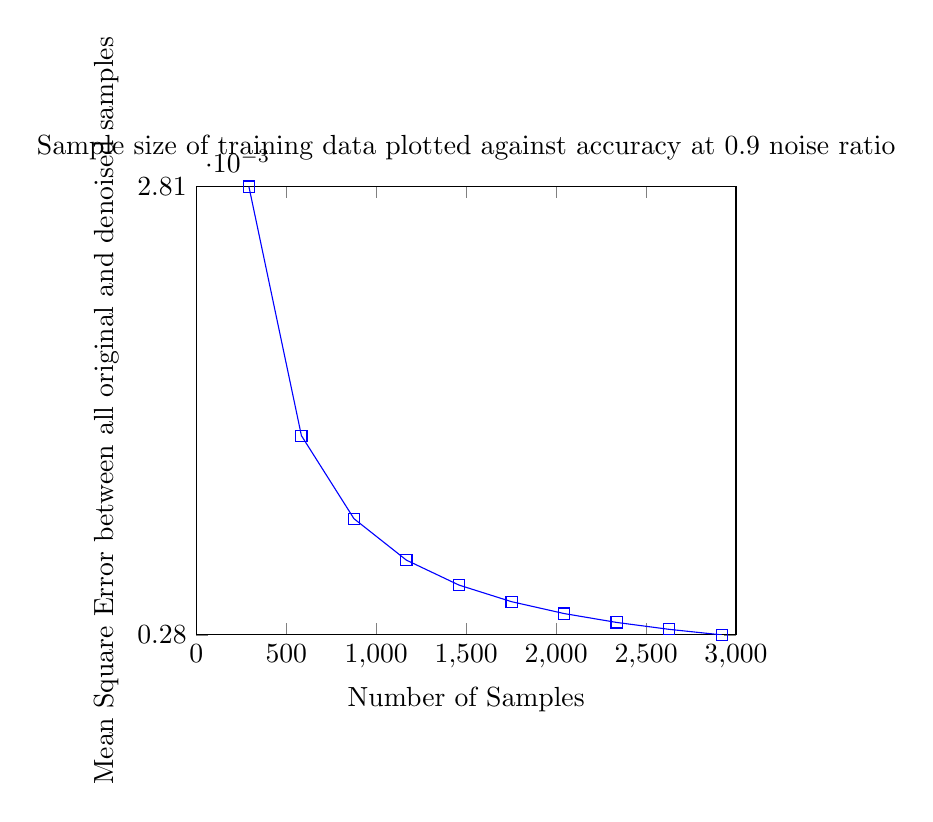
\begin{tikzpicture}
\begin{axis}[
title={Sample size of training data plotted against accuracy at 0.9 noise ratio},
xlabel={Number of Samples},
ylabel={Mean Square Error between all original and denoised samples},
xmin=0, xmax=3000,
ymin=0.00027774120470735417, ymax=0.002810755859915238,
xtick={0,500,1000,1500,2000,2500,3000},
ytick={0.00027774120470735417,0.002810755859915238,0.0053437705151231215,0.007876785170331005,0.01040979982553889,0.012942814480746774,0.015475829135954657,0.01800884379116254,0.020541858446370423,0.023074873101578307,0.025607887756786192},
legend pos=north west,
ymajorgrids=true,
grid style=dashed,
]

\addplot[
color=blue,
mark=square,
]
coordinates {

(292, 0.002810755859915238)
(584, 0.0014034958313624058)
(876, 0.0009344002106203093)
(1168, 0.0006998788255352679)
(1460, 0.0005591725354275189)
(1752, 0.00046537419594282626)
(2044, 0.0003983882648928203)
(2336, 0.0003481508666375487)
(2628, 0.0003090884367999383)
(2921, 0.00027774120470735417)
    };
\end{axis}
\end{tikzpicture}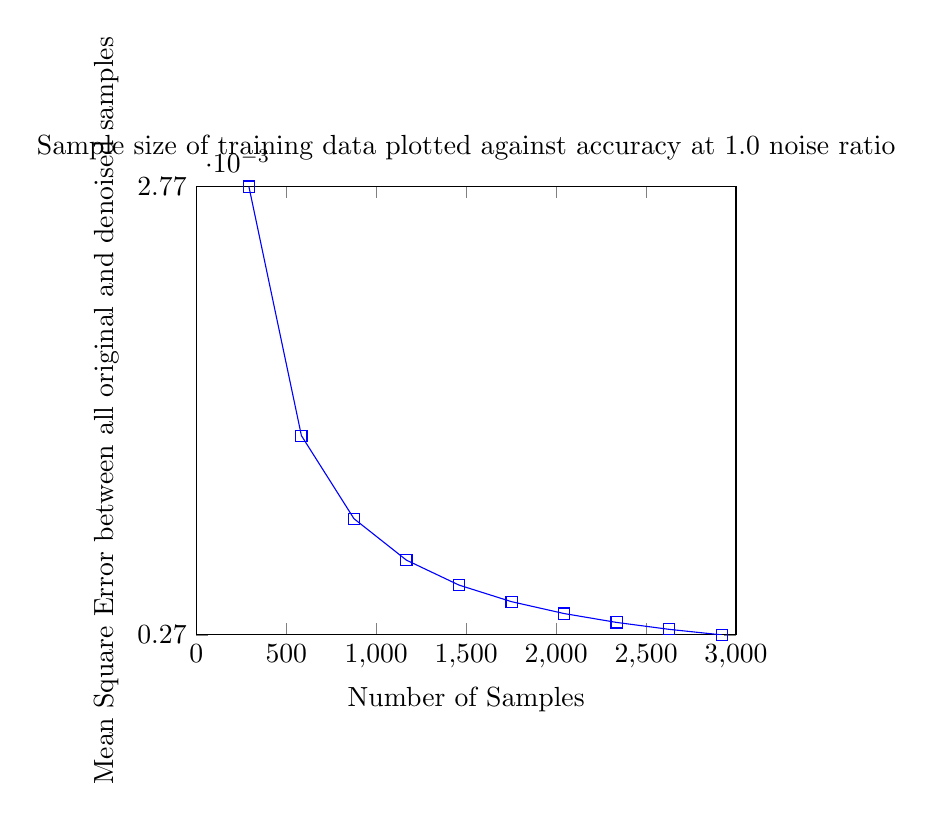
\begin{tikzpicture}
\begin{axis}[
title={Sample size of training data plotted against accuracy at 1.0 noise ratio},
xlabel={Number of Samples},
ylabel={Mean Square Error between all original and denoised samples},
xmin=0, xmax=3000,
ymin=0.00027458621394151273, ymax=0.002774971613690315,
xtick={0,500,1000,1500,2000,2500,3000},
ytick={0.00027458621394151273,0.002774971613690315,0.005275357013439117,0.007775742413187918,0.010276127812936721,0.012776513212685523,0.015276898612434324,0.01777728401218313,0.02027766941193193,0.022778054811680732,0.025278440211429536},
legend pos=north west,
ymajorgrids=true,
grid style=dashed,
]

\addplot[
color=blue,
mark=square,
]
coordinates {

(292, 0.002774971613690315)
(584, 0.0013858503553782963)
(876, 0.0009228032220743361)
(1168, 0.0006912948179328198)
(1460, 0.0005524029044274213)
(1752, 0.00045981955465859286)
(2044, 0.0003936897326656194)
(2336, 0.0003441036721892673)
(2628, 0.0003055340523879617)
(2921, 0.00027458621394151273)
    };
\end{axis}
\end{tikzpicture}



\end{document}
